\subsubsection{Resolution}
The energy resolution describes how well the detector can resolve detected photons of different energies. A detector with low resolution results in broad peaks which can cover smaller peaks, making them harder to detect.

\begin{figure}[H]
    \centering
    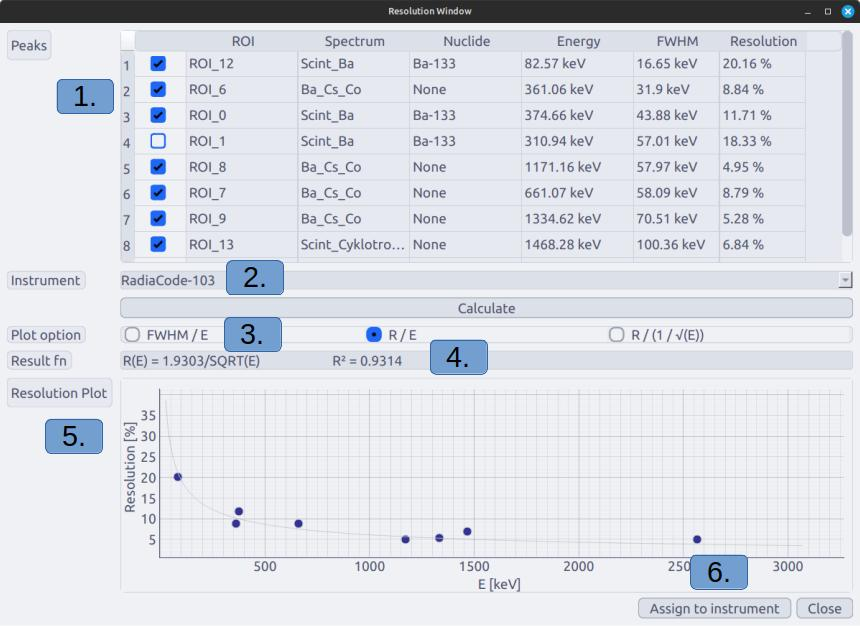
\includegraphics[width = .9\linewidth]{images/interface/gtools_resolution.jpg}
    \caption{Resolution window with several different spectra measured with a 3"x3" NaI(Tl) scintillator loaded. Using \texttt{Tabbed Spectrum View} so the ROIs are only evaluating one spectrum each.}
    \label{fig:gtools_resolution}

    \begin{flushleft}
        \begin{enumerate}
            \item Fitted peaks from all loaded spectra and ROIs. A ROI without a fit can not be included. Unchecked entries will be ignored in the calculation.
            \item Instrument to be given the calculation result. Can be Unique or Generic.
            \item Options for how the calculation results should be plotted. These do not affect the results, only the view.
            \item The resolution function, coefficients are in arbitrary units and not \% (\% = au * 100). The $R^2$ value of the fitted function compared with the data points.
            \item Assign the calculation resolution calibration to the instrument set in (2.).
        \end{enumerate}
    \end{flushleft}
\end{figure}